\documentclass[11pt,a4paper]{article}

\usepackage[utf8]{inputenc}
\usepackage[T1]{fontenc}
\usepackage[english]{babel}
\usepackage{lmodern}

\usepackage{geometry}
\geometry{
    top=2.5cm,
    bottom=2.5cm,
    left=2.5cm,
    right=2.5cm
}

\usepackage{amsmath,amssymb}
\usepackage{booktabs}
\usepackage{array}
\usepackage{graphicx}
\usepackage{listings}
\usepackage{xcolor}
\usepackage{fancyhdr}
\usepackage{hyperref}

\pagestyle{fancy}
\fancyhf{}
\rhead{\textit{Practical 4: Classification Models}}
\lhead{\textit{Data Science --- ETSINF (UPV)}}
\cfoot{\thepage}

\lstset{
    language=R,
    basicstyle=\ttfamily\footnotesize,
    keywordstyle=\color{blue}\bfseries,
    commentstyle=\color{gray}\itshape,
    stringstyle=\color{teal},
    numbers=none,
    frame=lines,
    breaklines=true,
    breakatwhitespace=true,
    showstringspaces=false,
    captionpos=b,
    tabsize=2
}

\title{\textbf{Practical 4: Classification Models}\\[0.4ex] \Large Data Science (CDA) --- Academic Lab Report}
\author{\textbf{Enrique Sopeña} \\ 
Máster Universitari en Enginyeria Informàtica (MUIInf) \\
Escola Tècnica Superior d'Enginyeria Informàtica (ETSINF) \\ 
Universitat Politècnica de València}
\date{\today}


\setlength{\headheight}{14pt}
\lstdefinestyle{console}{
    language={},
    basicstyle=\ttfamily\scriptsize,
    frame=single,
    keywordstyle=\color{black},
    commentstyle=\color{black},
    stringstyle=\color{black},
    columns=fullflexible,
    keepspaces=true
}
\begin{document}
\maketitle

\begin{abstract}
  This report presents a classification study of the Wine dataset using decision trees in R. The 178 observations are randomly divided into 133 training cases and 45 test cases. A baseline tree is fitted with \texttt{rpart}, compared with a tree trained on the full dataset, and evaluated through class probabilities, predicted labels, and a confusion matrix. Nine parameter configurations are then assessed using internal cross-validation on the training set. Both the baseline and the selected tree correctly classify 40 of the 45 test observations, yielding an accuracy of 88.89\%. The selected configuration improves the recorded cross-validation result but does not improve test accuracy. Code excerpts and recorded console output support the analysis throughout the report.
\end{abstract}

\vspace{0.8em}
\hrule
\vspace{1em}

\section{Introduction and Experimental Setup}
The Wine dataset supplied with Practical~4 contains chemical measurements of wines from three classes grown in the same region in Italy. Each observation includes a class label and 13 predictors: alcohol, malic acid, ash, alcalinity of ash, magnesium, total phenols, flavanoids, nonflavanoid phenols, proanthocyanins, colour intensity, hue, OD280/OD315 of diluted wines, and proline. The objective is to predict the wine class from these measurements using a decision tree.

All experiments are implemented sequentially in \texttt{pract4.R}, with paths relative to the practical's root directory. The input file is \texttt{dataset/wine.data.txt}. Generated files are stored in \texttt{outputs/}, including the tree visualisations and the execution log. The seed is set to 123 for the random split and before model fitting. Numerical results in this report come from the supplied final execution log; percentages discussed in the text are calculated from its counts.

\newpage
\section{Exercise 1: Random Train/Test Split}
\subsection{Objective and Implementation}
The first exercise creates a random 75\%/25\% train/test split. Column names are assigned explicitly, and the target is converted to a factor so that its values represent classes rather than a continuous response. Sampling without replacement selects the training rows, while the remaining rows form the test set. This is a simple random split, without stratification.
\begin{lstlisting}
wine <- read.table("dataset/wine.data.txt", header = FALSE, sep = ",")

names(wine) <- c(
  "class", "alco", "ma", "ash", "alc", "mg", "tp",
  "flav", "noflav", "proa", "col", "hue", "od", "prol"
)

wine$class <- as.factor(wine$class)

# Fix the seed to reproduce the split; sample without replacement
# so that training and test observations cannot overlap.
set.seed(123)

train_indices <- sample(
  seq_len(nrow(wine)),
  size = floor(0.75 * nrow(wine)),
  replace = FALSE
)

wine_train <- wine[train_indices, ]
wine_test <- wine[-train_indices, ]

split_summary <- data.frame(
  Set = c("Training", "Test"),
  Observations = c(nrow(wine_train), nrow(wine_test)),
  Percentage = round(
    100 * c(nrow(wine_train), nrow(wine_test)) / nrow(wine), 2
  )
)

print(split_summary, row.names = FALSE)

class_distribution <- cbind(
  Full = table(wine$class),
  Training = table(wine_train$class),
  Test = table(wine_test$class)
)

print(class_distribution)
\end{lstlisting}

\subsection{Results and Discussion}
\par\noindent\begin{minipage}{\linewidth}
  \begin{lstlisting}[style=console]
Set Observations Percentage
 Training          133      74.72
     Test           45      25.28
  Full Training Test
1   59       45   14
2   71       51   20
3   48       37   11
\end{lstlisting}
\end{minipage}\par

Since $0.75\times178=133.5$, taking the floor produces 133 training observations and 45 test observations. The realised proportions are therefore 74.72\% and 25.28\%. All three classes are represented in both subsets. The training counts are 45, 51, and 37, while the test counts are 14, 20, and 11 for classes 1, 2, and 3, respectively. The disjoint row selection ensures that no observation belongs to both subsets.

\section{Exercise 2: Training a Classification Tree}
\subsection{Objective and Implementation}
A baseline classification tree is fitted using only the training set. The formula \texttt{class \textasciitilde{} .} includes all 13 predictors, and \texttt{method = "class"} requests classification. The remaining tree controls retain their default values.
\begin{lstlisting}
library(rpart)

# Use the training set only, keeping the test set for evaluation.
set.seed(123)

model_train <- rpart(
  class ~ .,
  data = wine_train,
  method = "class"
)

print(model_train)
printcp(model_train)
\end{lstlisting}

\subsection{Results and Discussion}
The fitted tree is printed below. Each node reports its condition, sample size, misclassification loss, predicted class, and class probabilities. An asterisk marks a terminal node.
\par\noindent\begin{minipage}{\linewidth}
  \begin{lstlisting}[style=console]
n= 133 

node), split, n, loss, yval, (yprob)
      * denotes terminal node

1) root 133 82 2 (0.33834586 0.38345865 0.27819549)  
  2) flav>=2.31 56 11 1 (0.80357143 0.19642857 0.00000000)  
    4) prol>=670 46  1 1 (0.97826087 0.02173913 0.00000000) *
    5) prol< 670 10  0 2 (0.00000000 1.00000000 0.00000000) *
  3) flav< 2.31 77 37 2 (0.00000000 0.51948052 0.48051948)  
    6) col< 3.825 37  0 2 (0.00000000 1.00000000 0.00000000) *
    7) col>=3.825 40  3 3 (0.00000000 0.07500000 0.92500000) *

Classification tree:
rpart(formula = class ~ ., data = wine_train, method = "class")

Variables actually used in tree construction:
[1] col  flav prol

Root node error: 82/133 = 0.61654

n= 133 

       CP nsplit rel error  xerror     xstd
1 0.41463      0   1.00000 1.00000 0.068384
2 0.12195      2   0.17073 0.32927 0.056571
3 0.01000      3   0.04878 0.15854 0.041766
\end{lstlisting}
\end{minipage}\par

The tree uses flavanoids (\texttt{flav}), proline (\texttt{prol}), and colour intensity (\texttt{col}). It has three splits and four terminal nodes. Wines with \texttt{flav} at least 2.31 are separated using a proline threshold of 670; wines below that flavanoid threshold are separated using a colour intensity threshold of 3.825.

The terminal-node losses sum to $1+0+0+3=4$, giving a training accuracy of $129/133=96.99\%$. The root predicts the majority class, class~2, and would misclassify $133-51=82$ observations without any splits. Consequently, the final relative training error is $4/82=0.04878$. This value is relative to the root-node error, rather than the fraction of misclassified training cases. Likewise, \texttt{xerror} is the relative cross-validation error, and \texttt{xstd} is its estimated standard error; neither is a test-set result.

\section{Exercise 3: Visualisation and Full-Dataset Comparison}
\subsection{Objective and Implementation}
A second tree is fitted on all 178 observations to examine how its structure differs from the training-only model. It is used solely for this descriptive comparison, not to predict the held-out test cases in the following exercises. The two visualisations are saved as separate pages of \texttt{outputs/decision\_trees.pdf}. Figures~\ref{fig:training-tree} and~\ref{fig:full-tree} reproduce these visualisations alongside the numerical and textual results.
\begin{lstlisting}
dir.create("outputs", showWarnings = FALSE)

set.seed(123)

model_full <- rpart(
  class ~ .,
  data = wine,
  method = "class"
)

pdf("outputs/decision_trees.pdf", width = 10, height = 7)

plot(
  model_train,
  main = "Decision tree: training set",
  uniform = TRUE,
  margin = 0.1
)
text(model_train, use.n = TRUE, all = FALSE, cex = 0.8)

plot(
  model_full,
  main = "Decision tree: full dataset",
  uniform = TRUE,
  margin = 0.1
)
text(model_full, use.n = TRUE, all = FALSE, cex = 0.8)

invisible(dev.off())

cat("\n--- Tree trained on the full dataset ---\n")
print(model_full)
printcp(model_full)

tree_summary <- function(model) {
  leaves <- model$frame$var == "<leaf>"

  c(
    Observations = model$frame$n[1],
    Splits = sum(!leaves),
    Leaves = sum(leaves),
    Training_errors = sum(model$frame$dev[leaves])
  )
}

comparison <- rbind(
  Training_set = tree_summary(model_train),
  Full_dataset = tree_summary(model_full)
)

cat("\n--- Tree comparison ---\n")
print(comparison)
\end{lstlisting}

\clearpage
\subsection{Decision Tree Visualisations}
The training-only tree has four leaves, whereas the full-dataset tree has five. Each leaf shows its predicted class and the counts for classes 1, 2, and 3, in that order.

\begin{figure}[htbp]
  \centering
  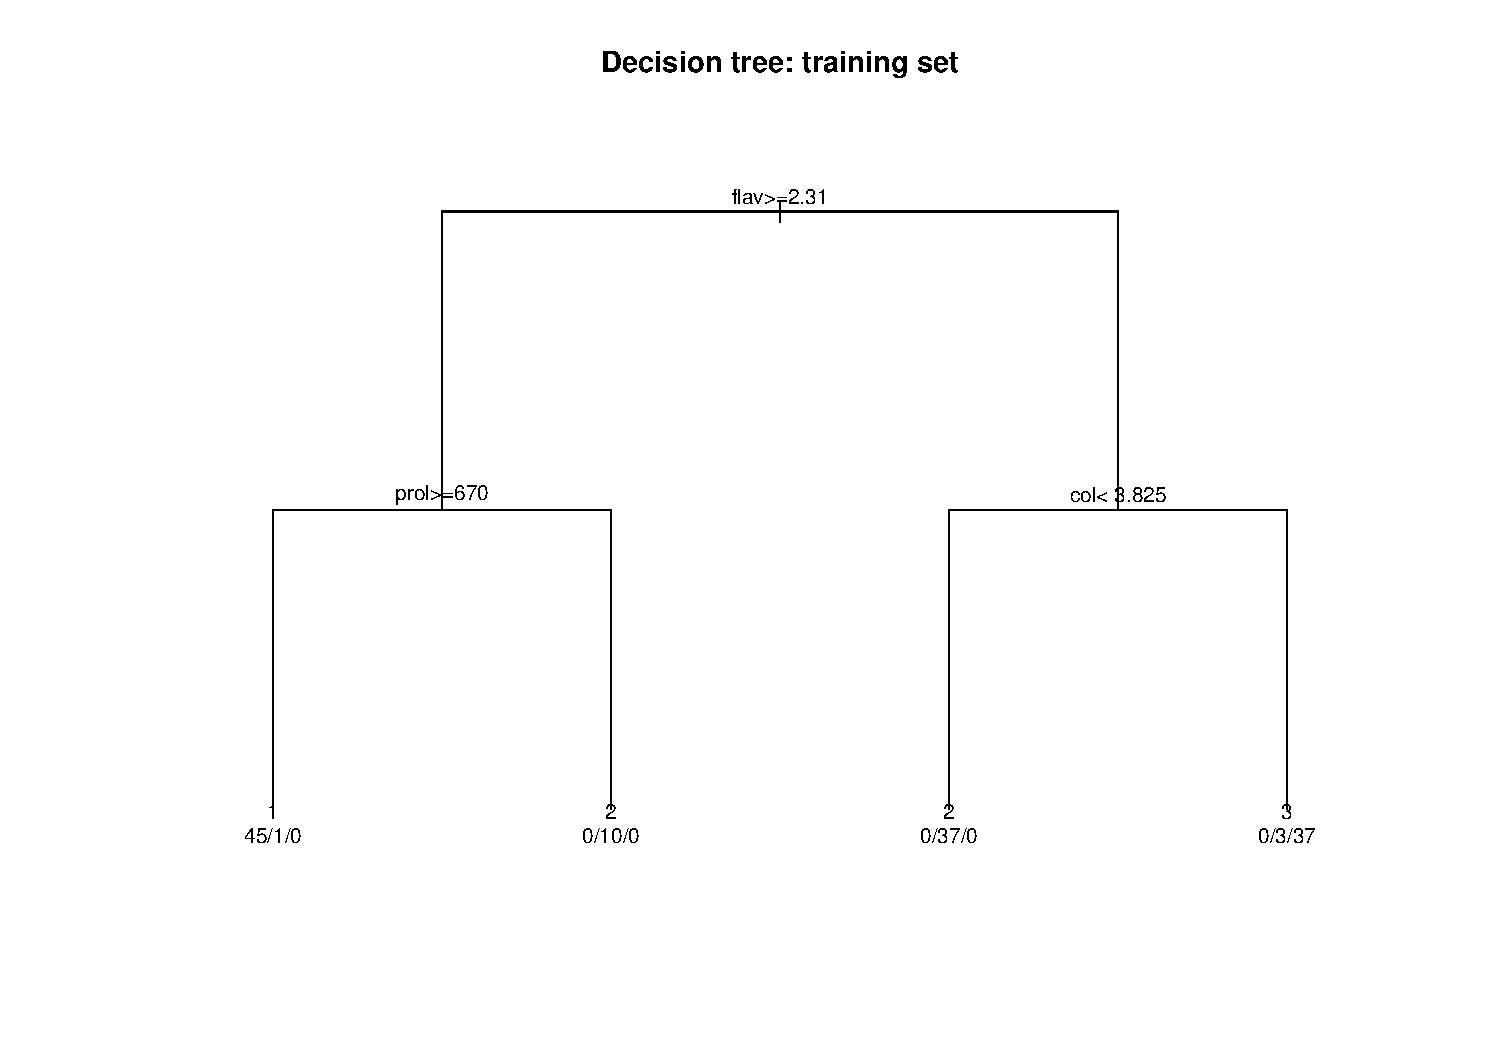
\includegraphics[page=1,width=0.78\textwidth,trim=35 45 35 15,clip]{../outputs/decision_trees.pdf}
  \caption{Decision tree fitted to the 133 training observations.}
  \label{fig:training-tree}
  \vspace{1em}
  \includegraphics[page=2,width=0.78\textwidth,trim=35 45 35 15,clip]{../outputs/decision_trees.pdf}
  \caption{Decision tree fitted to all 178 observations, used for structural comparison.}
  \label{fig:full-tree}
\end{figure}
\clearpage

\subsection{Results and Discussion}
The full-dataset tree has the following structure:
\par\noindent\begin{minipage}{\linewidth}
  \begin{lstlisting}[style=console]
n= 178 

node), split, n, loss, yval, (yprob)
      * denotes terminal node

 1) root 178 107 2 (0.33146067 0.39887640 0.26966292)  
   2) prol>=755 67  10 1 (0.85074627 0.05970149 0.08955224)  
     4) flav>=2.165 59   2 1 (0.96610169 0.03389831 0.00000000) *
     5) flav< 2.165 8   2 3 (0.00000000 0.25000000 0.75000000) *
   3) prol< 755 111  44 2 (0.01801802 0.60360360 0.37837838)  
     6) od>=2.115 65   4 2 (0.03076923 0.93846154 0.03076923) *
     7) od< 2.115 46   6 3 (0.00000000 0.13043478 0.86956522)  
      14) hue>=0.9 7   2 2 (0.00000000 0.71428571 0.28571429) *
      15) hue< 0.9 39   1 3 (0.00000000 0.02564103 0.97435897) *
\end{lstlisting}
\end{minipage}\par
\par\noindent\begin{minipage}{\linewidth}
  \begin{lstlisting}[style=console]
Observations Splits Leaves Training_errors
Training_set          133      3      4               4
Full_dataset          178      4      5              11
\end{lstlisting}
\end{minipage}\par

The root split changes from \texttt{flav >= 2.31} in the training-only tree to \texttt{prol >= 755} in the full-dataset tree. Both models use flavanoids and proline, but their thresholds and the order of their splits differ. The full-dataset model additionally uses \texttt{od} and \texttt{hue}, whereas the training-only model uses \texttt{col}. Its four splits produce five leaves, compared with three splits and four leaves in the baseline.

The full-dataset tree makes 11 errors on its 178 fitting observations, corresponding to a resubstitution error of 6.18\%. The baseline makes four errors on 133 fitting observations, or 3.01\%. These values describe fit to different datasets and cannot establish which model generalises better. The structural differences demonstrate that the fitted decision rules depend on the observations available during training. Both pages of the generated PDF were checked for readable labels and agreement with the console output.

\section{Exercise 4: Probabilities and Predicted Classes}
\subsection{Objective and Implementation}
Predictions for the test set are generated with the training-only model. For this classification tree, the default prediction output is a matrix of class probabilities; specifying \texttt{type = "class"} returns class labels. The two outputs are retained in separate variables.
\begin{lstlisting}
pred_prob <- predict(model_train, newdata = wine_test)

pred_class <- predict(
  model_train,
  newdata = wine_test,
  type = "class"
)

cat("\n--- Predicted probabilities ---\n")
print(pred_prob)

cat("\n--- Predicted class labels ---\n")
print(pred_class)

cat("\n--- Prediction output structure ---\n")
str(pred_prob)
str(pred_class)
\end{lstlisting}

\subsection{Results and Discussion}
The recorded structures show the difference between the outputs:
\par\noindent\begin{minipage}{\linewidth}
  \begin{lstlisting}[style=console]
num [1:45, 1:3] 0.978 0.978 0.978 0.978 0.978 ...
 - attr(*, "dimnames")=List of 2
  ..$ : chr [1:45] "1" "2" "3" "10" ...
  ..$ : chr [1:3] "1" "2" "3"
 Factor w/ 3 levels "1","2","3": 1 1 1 1 1 1 1 3 1 1 ...
 - attr(*, "names")= chr [1:45] "1" "2" "3" "10" ...
\end{lstlisting}
\end{minipage}\par

The probability matrix has 45 rows and three columns, one per class. For example, original row~1 receives probabilities $(0.9782609, 0.02173913, 0)$ and is assigned class~1. Original row~28 receives $(0, 0.075, 0.925)$ and is assigned class~3. The factor contains one predicted class per test observation; under the default loss settings used here, it selects the class with the largest probability. Observation names retain the original dataset row indices.

Observations reaching the same leaf receive the same empirical class distribution. Both leaves predicting class~2 are pure in training and therefore return $(0,1,0)$. A probability of one here describes the training leaf; it does not guarantee that a new observation is correctly classified. The complete predictions are reproduced in the appendix.

\section{Exercise 5: Test-Set Evaluation}
\subsection{Objective and Implementation}
A confusion matrix compares the predicted labels with the actual test classes. Rows correspond to predictions and columns to actual classes. Summing the diagonal yields the number of correct predictions.
\begin{lstlisting}
confusion_matrix <- table(
  Predicted = pred_class,
  Actual = wine_test$class
)

cat("\n--- Confusion matrix ---\n")
print(confusion_matrix)

correct <- sum(diag(confusion_matrix))
total <- sum(confusion_matrix)

test_performance <- data.frame(
  Observations = total,
  Correct = correct,
  Incorrect = total - correct,
  Accuracy = correct / total,
  Error_rate = 1 - correct / total
)

cat("\n--- Test performance ---\n")
print(test_performance, row.names = FALSE)
\end{lstlisting}

\subsection{Results and Discussion}
\par\noindent\begin{minipage}{\linewidth}
  \begin{lstlisting}[style=console]
Actual
Predicted  1  2  3
        1 13  3  0
        2  0 16  0
        3  1  1 11

--- Test performance ---
 Observations Correct Incorrect  Accuracy Error_rate
           45      40         5 0.8888889  0.1111111
\end{lstlisting}
\end{minipage}\par

The test accuracy and error rate are
\[
  \mathrm{Accuracy}=\frac{13+16+11}{45}=\frac{40}{45}=88.89\%,
  \qquad
  \mathrm{Error\ rate}=\frac{5}{45}=11.11\%.
\]
For class~1, 13 of 14 wines are correctly identified and one is assigned to class~3. For class~2, 16 of 20 are correct, three are assigned to class~1, and one to class~3. All 11 actual class~3 wines are correctly classified, although the model also assigns two wines from other classes to class~3.

Test accuracy is lower than training accuracy (88.89\% versus 96.99\%). This difference is consistent with a weaker fit to unseen observations, but a single split with 45 test cases does not establish the extent of overfitting. The test result provides the baseline for the final exercise.

\section{Exercise 6: Parameter Tuning and Model Comparison}
\subsection{Objective and Implementation}
Nine configurations combine \texttt{minsplit} values of 10, 20, and 30 with \texttt{maxdepth} values of 2, 3, and 5. The former controls the minimum node size for attempting a split, while the latter limits tree depth. Since \texttt{minbucket} is not specified, its default is derived as \texttt{round(minsplit/3)}; the corresponding minimum leaf sizes are 3, 7, and 10. Thus, varying \texttt{minsplit} also changes this default leaf-size constraint.

Each candidate is grown with \texttt{cp = 0} within these constraints and assessed using ten-fold internal cross-validation. The complexity-table row with the smallest relative cross-validation error determines its pruning parameter. Ties favour fewer splits. The same criterion selects the final candidate across configurations; any remaining tie follows their order in the grid. Test labels are not used by this selection procedure.
\begin{lstlisting}
parameter_grid <- expand.grid(
  minsplit = c(10, 20, 30),
  maxdepth = c(2, 3, 5)
)

candidate_models <- vector("list", nrow(parameter_grid))
tuning_results <- parameter_grid

for (i in seq_len(nrow(parameter_grid))) {
  set.seed(123)

  candidate <- rpart(
    class ~ .,
    data = wine_train,
    method = "class",
    control = rpart.control(
      minsplit = parameter_grid$minsplit[i],
      maxdepth = parameter_grid$maxdepth[i],
      cp = 0,
      xval = 10
    )
  )

  # Select pruning complexity by cross-validation, preferring
  # fewer splits when validation errors are tied.
  cp_table <- candidate$cptable
  best_row <- order(
    cp_table[, "xerror"],
    cp_table[, "nsplit"]
  )[1]

  best_cp <- cp_table[best_row, "CP"]

  candidate_models[[i]] <- prune(candidate, cp = best_cp)

  tuning_results$CP[i] <- best_cp
  tuning_results$Splits[i] <- cp_table[best_row, "nsplit"]
  tuning_results$CV_relative_error[i] <- cp_table[best_row, "xerror"]
}

cat("\n--- Cross-validation results ---\n")
print(tuning_results, row.names = FALSE)

best_index <- order(
  tuning_results$CV_relative_error,
  tuning_results$Splits
)[1]

model_tuned <- candidate_models[[best_index]]

cat("\n--- Selected configuration ---\n")
print(tuning_results[best_index, ], row.names = FALSE)

cat("\n--- Selected tree ---\n")
print(model_tuned)
\end{lstlisting}

\subsection{Cross-Validation Results}
\par\noindent\begin{minipage}{\linewidth}
  \begin{lstlisting}[style=console]
minsplit maxdepth CP Splits CV_relative_error
       10        2  0      3         0.1585366
       20        2  0      3         0.1829268
       30        2  0      3         0.2560976
       10        3  0      4         0.1341463
       20        3  0      3         0.1585366
       30        3  0      3         0.2682927
       10        5  0      4         0.1341463
       20        5  0      3         0.1585366
       30        5  0      3         0.2682927

--- Selected configuration ---
 minsplit maxdepth CP Splits CV_relative_error
       10        3  0      4         0.1341463
\end{lstlisting}
\end{minipage}\par

The selected configuration is \texttt{minsplit = 10}, \texttt{maxdepth = 3}, and \texttt{cp = 0}, with four splits. The configuration with \texttt{maxdepth = 5} has the same error and split count, so the earlier grid entry is retained. The relative cross-validation error is 0.1341463, below the baseline's recorded 0.15854. This is a model-selection result, not an independent estimate of the selected model's performance.

All retained configurations have \texttt{CP = 0}. Although the implementation calls \texttt{prune()}, no positive-complexity pruning is selected: the final tree retains the candidate's branches. It would therefore be incorrect to attribute the result to a successful reduction in tree size through pruning.

\subsection{Selected Tree and Test Evaluation}
\par\noindent\begin{minipage}{\linewidth}
  \begin{lstlisting}[style=console]
n= 133 

node), split, n, loss, yval, (yprob)
      * denotes terminal node

 1) root 133 82 2 (0.33834586 0.38345865 0.27819549)  
   2) flav>=2.31 56 11 1 (0.80357143 0.19642857 0.00000000)  
     4) prol>=670 46  1 1 (0.97826087 0.02173913 0.00000000) *
     5) prol< 670 10  0 2 (0.00000000 1.00000000 0.00000000) *
   3) flav< 2.31 77 37 2 (0.00000000 0.51948052 0.48051948)  
     6) col< 3.825 37  0 2 (0.00000000 1.00000000 0.00000000) *
     7) col>=3.825 40  3 3 (0.00000000 0.07500000 0.92500000)  
      14) flav>=1.4 3  0 2 (0.00000000 1.00000000 0.00000000) *
      15) flav< 1.4 37  0 3 (0.00000000 0.00000000 1.00000000) *
\end{lstlisting}
\end{minipage}\par

The selected tree adds a split at \texttt{flav = 1.4} within the branch satisfying \texttt{flav < 2.31} and \texttt{col >= 3.825}. The previous leaf contained three class~2 wines and 37 class~3 wines. The new split separates these training cases into two pure leaves, reducing the total training loss from four to one. The tree now has five leaves.

The selected model is then evaluated on the same test set:
\begin{lstlisting}
# Evaluate the selected model on test data only after tuning.
pred_tuned <- predict(
  model_tuned,
  newdata = wine_test,
  type = "class"
)

confusion_tuned <- table(
  Predicted = pred_tuned,
  Actual = wine_test$class
)

cat("\n--- Tuned model confusion matrix ---\n")
print(confusion_tuned)

model_comparison <- data.frame(
  Model = c("Default tree", "Tuned tree"),
  Correct = c(
    sum(pred_class == wine_test$class),
    sum(pred_tuned == wine_test$class)
  ),
  Incorrect = c(
    sum(pred_class != wine_test$class),
    sum(pred_tuned != wine_test$class)
  ),
  Accuracy = c(
    mean(pred_class == wine_test$class),
    mean(pred_tuned == wine_test$class)
  )
)

cat("\n--- Test performance comparison ---\n")
print(model_comparison, row.names = FALSE)
\end{lstlisting}
\par\noindent\begin{minipage}{\linewidth}
  \begin{lstlisting}[style=console]
Actual
Predicted  1  2  3
        1 13  3  0
        2  1 17  1
        3  0  0 10

--- Test performance comparison ---
        Model Correct Incorrect  Accuracy
 Default tree      40         5 0.8888889
   Tuned tree      40         5 0.8888889
\end{lstlisting}
\end{minipage}\par

Both models correctly classify 40 of 45 observations, so test accuracy remains 88.89\%. The tuned model identifies 17 rather than 16 of the 20 actual class~2 wines, but identifies 10 rather than 11 of the actual class~3 wines. Class~1 still has 13 correct predictions. The additional split changes the distribution of errors without reducing their total.

\section{Conclusions}
The practical demonstrates the complete workflow of splitting data, training classification trees, inspecting their decision rules, generating predictions, and evaluating held-out cases. Training on the full dataset changes the root variable, thresholds, and tree structure, illustrating the dependence of decision trees on the available training observations.

Parameter tuning improves the recorded cross-validation result and training fit, but does not improve test accuracy: both evaluated models achieve 88.89\%. The baseline reaches this result with one fewer split. The experiment therefore provides no test-set evidence that the additional complexity improves prediction. These conclusions apply to the fixed split studied here, rather than establishing a general ranking across other samples or partitions.

\newpage
\appendix
\section*{Appendix: Complete Sequential Execution Log}
\addcontentsline{toc}{section}{Appendix: Complete Sequential Execution Log}
The complete supplied console output from \texttt{pract4.R}, saved in \texttt{outputs/pract4-output.txt}, is reproduced below without changing its numerical values.
\begin{lstlisting}[style=console]
      Set Observations Percentage
 Training          133      74.72
     Test           45      25.28
  Full Training Test
1   59       45   14
2   71       51   20
3   48       37   11
n= 133 

node), split, n, loss, yval, (yprob)
      * denotes terminal node

1) root 133 82 2 (0.33834586 0.38345865 0.27819549)  
  2) flav>=2.31 56 11 1 (0.80357143 0.19642857 0.00000000)  
    4) prol>=670 46  1 1 (0.97826087 0.02173913 0.00000000) *
    5) prol< 670 10  0 2 (0.00000000 1.00000000 0.00000000) *
  3) flav< 2.31 77 37 2 (0.00000000 0.51948052 0.48051948)  
    6) col< 3.825 37  0 2 (0.00000000 1.00000000 0.00000000) *
    7) col>=3.825 40  3 3 (0.00000000 0.07500000 0.92500000) *

Classification tree:
rpart(formula = class ~ ., data = wine_train, method = "class")

Variables actually used in tree construction:
[1] col  flav prol

Root node error: 82/133 = 0.61654

n= 133 

       CP nsplit rel error  xerror     xstd
1 0.41463      0   1.00000 1.00000 0.068384
2 0.12195      2   0.17073 0.32927 0.056571
3 0.01000      3   0.04878 0.15854 0.041766

--- Tree trained on the full dataset ---
n= 178 

node), split, n, loss, yval, (yprob)
      * denotes terminal node

 1) root 178 107 2 (0.33146067 0.39887640 0.26966292)  
   2) prol>=755 67  10 1 (0.85074627 0.05970149 0.08955224)  
     4) flav>=2.165 59   2 1 (0.96610169 0.03389831 0.00000000) *
     5) flav< 2.165 8   2 3 (0.00000000 0.25000000 0.75000000) *
   3) prol< 755 111  44 2 (0.01801802 0.60360360 0.37837838)  
     6) od>=2.115 65   4 2 (0.03076923 0.93846154 0.03076923) *
     7) od< 2.115 46   6 3 (0.00000000 0.13043478 0.86956522)  
      14) hue>=0.9 7   2 2 (0.00000000 0.71428571 0.28571429) *
      15) hue< 0.9 39   1 3 (0.00000000 0.02564103 0.97435897) *

Classification tree:
rpart(formula = class ~ ., data = wine, method = "class")

Variables actually used in tree construction:
[1] flav hue  od   prol

Root node error: 107/178 = 0.60112

n= 178 

        CP nsplit rel error  xerror     xstd
1 0.495327      0   1.00000 1.00000 0.061056
2 0.317757      1   0.50467 0.50467 0.057321
3 0.056075      2   0.18692 0.32710 0.049557
4 0.028037      3   0.13084 0.28037 0.046676
5 0.010000      4   0.10280 0.26168 0.045397

--- Tree comparison ---
             Observations Splits Leaves Training_errors
Training_set          133      3      4               4
Full_dataset          178      4      5              11

--- Predicted probabilities ---
            1          2     3
1   0.9782609 0.02173913 0.000
2   0.9782609 0.02173913 0.000
3   0.9782609 0.02173913 0.000
10  0.9782609 0.02173913 0.000
15  0.9782609 0.02173913 0.000
18  0.9782609 0.02173913 0.000
20  0.9782609 0.02173913 0.000
28  0.0000000 0.07500000 0.925
29  0.9782609 0.02173913 0.000
33  0.9782609 0.02173913 0.000
45  0.9782609 0.02173913 0.000
49  0.9782609 0.02173913 0.000
56  0.9782609 0.02173913 0.000
58  0.9782609 0.02173913 0.000
61  0.0000000 1.00000000 0.000
65  0.0000000 1.00000000 0.000
66  0.9782609 0.02173913 0.000
68  0.0000000 0.07500000 0.925
70  0.0000000 1.00000000 0.000
75  0.0000000 1.00000000 0.000
82  0.9782609 0.02173913 0.000
88  0.0000000 1.00000000 0.000
95  0.0000000 1.00000000 0.000
98  0.0000000 1.00000000 0.000
100 0.0000000 1.00000000 0.000
101 0.0000000 1.00000000 0.000
102 0.0000000 1.00000000 0.000
104 0.0000000 1.00000000 0.000
110 0.9782609 0.02173913 0.000
111 0.0000000 1.00000000 0.000
120 0.0000000 1.00000000 0.000
124 0.0000000 1.00000000 0.000
128 0.0000000 1.00000000 0.000
129 0.0000000 1.00000000 0.000
132 0.0000000 0.07500000 0.925
133 0.0000000 0.07500000 0.925
134 0.0000000 0.07500000 0.925
136 0.0000000 0.07500000 0.925
139 0.0000000 0.07500000 0.925
144 0.0000000 0.07500000 0.925
151 0.0000000 0.07500000 0.925
155 0.0000000 0.07500000 0.925
157 0.0000000 0.07500000 0.925
164 0.0000000 0.07500000 0.925
178 0.0000000 0.07500000 0.925

--- Predicted class labels ---
  1   2   3  10  15  18  20  28  29  33  45  49  56  58  61  65  66  68  70  75 
  1   1   1   1   1   1   1   3   1   1   1   1   1   1   2   2   1   3   2   2 
 82  88  95  98 100 101 102 104 110 111 120 124 128 129 132 133 134 136 139 144 
  1   2   2   2   2   2   2   2   1   2   2   2   2   2   3   3   3   3   3   3 
151 155 157 164 178 
  3   3   3   3   3 
Levels: 1 2 3

--- Prediction output structure ---
 num [1:45, 1:3] 0.978 0.978 0.978 0.978 0.978 ...
 - attr(*, "dimnames")=List of 2
  ..$ : chr [1:45] "1" "2" "3" "10" ...
  ..$ : chr [1:3] "1" "2" "3"
 Factor w/ 3 levels "1","2","3": 1 1 1 1 1 1 1 3 1 1 ...
 - attr(*, "names")= chr [1:45] "1" "2" "3" "10" ...

--- Confusion matrix ---
         Actual
Predicted  1  2  3
        1 13  3  0
        2  0 16  0
        3  1  1 11

--- Test performance ---
 Observations Correct Incorrect  Accuracy Error_rate
           45      40         5 0.8888889  0.1111111

--- Cross-validation results ---
 minsplit maxdepth CP Splits CV_relative_error
       10        2  0      3         0.1585366
       20        2  0      3         0.1829268
       30        2  0      3         0.2560976
       10        3  0      4         0.1341463
       20        3  0      3         0.1585366
       30        3  0      3         0.2682927
       10        5  0      4         0.1341463
       20        5  0      3         0.1585366
       30        5  0      3         0.2682927

--- Selected configuration ---
 minsplit maxdepth CP Splits CV_relative_error
       10        3  0      4         0.1341463

--- Selected tree ---
n= 133 

node), split, n, loss, yval, (yprob)
      * denotes terminal node

 1) root 133 82 2 (0.33834586 0.38345865 0.27819549)  
   2) flav>=2.31 56 11 1 (0.80357143 0.19642857 0.00000000)  
     4) prol>=670 46  1 1 (0.97826087 0.02173913 0.00000000) *
     5) prol< 670 10  0 2 (0.00000000 1.00000000 0.00000000) *
   3) flav< 2.31 77 37 2 (0.00000000 0.51948052 0.48051948)  
     6) col< 3.825 37  0 2 (0.00000000 1.00000000 0.00000000) *
     7) col>=3.825 40  3 3 (0.00000000 0.07500000 0.92500000)  
      14) flav>=1.4 3  0 2 (0.00000000 1.00000000 0.00000000) *
      15) flav< 1.4 37  0 3 (0.00000000 0.00000000 1.00000000) *

--- Tuned model confusion matrix ---
         Actual
Predicted  1  2  3
        1 13  3  0
        2  1 17  1
        3  0  0 10

--- Test performance comparison ---
        Model Correct Incorrect  Accuracy
 Default tree      40         5 0.8888889
   Tuned tree      40         5 0.8888889
\end{lstlisting}

\end{document}
